\section{Further research trends}
\subsection{Physical And Mental Aspects}

Ranasinghe, Nimesha and Do, Ellen Yi-Luen have developed a way to address the tastebuds using electrical stimulation \cite{Ranasinghe:2016:VSS:2984751.2985729}

Health care training for professional workers in health-care

People could be treated with games, regarding the profits of arcieving womething, and VR, the profit of feeling right in the middle of the happening

cyber sickness is a large field, witch should be researched because, weh the people dont move but the eyes tell the brain that they are moving, it becomes confused (similar to sea-sickness)

motivation of players: (talk)\footnote{"Gamer Motivation Profile Findings - \#GamesUR US Conference 2016" Quantic Foundry Website, March, 25., 2015, accessed November 05., 2016, \url{http://quanticfoundry.com/2016/04/07/gdc-talk/}}
\begin{itemize}
	\item action
	\item social
	\item mastery
	\item achievement
	\item immersion
	\item creativity
\end{itemize}

%\textcolor{gray}{\blindtext[3]}

\subsection{Physical Objects}

Using some similar technology to the iDummy\footnote{"IDummy" IDummy Product Website, 2015, accessed November 05., 2016, \url{http://www.idummy.com/}} one can create various objects of different size and shape. A user wearing a VR Headset can see a specific object and feel it as if it was the real thing. Using the technology developers can extend the realm of VR to one more dimension. Together with the technology~\cite{Azmandian:2016:HRD:2858036.2858226}

Using something similar to the modular tiles creating levels in portal (a 100x100 cm tile is attached to a robotic arm)

\begin{figure}
	\centering
	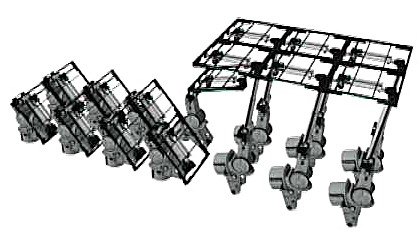
\includegraphics[width=0.9\columnwidth]{./figures/portallabrattest}
	\caption[Portal 2 : Lab Rat Panel Test]{Screenshot from the promotional video 'Portal 2 : Lab Rat Panel Test' (\ccbyncsa) of the game \textit{Portal 2 \textregistered\textcopyright} showing the general setup of floor panels mounted to robotic arms. This method enables developers to modify the structure of the floor at runtime.\footnotemark}~\label{fig:portallabrattest}
\end{figure}
\footnotetext{\textcopyright "Valve Software", [Online; accessed November 05., 2016],[Digitally revised] \url{https://www.youtube.com/watch?v=S7vFxs0ycn0}}

I can think of an application where the tiles are intelligently configured to 'disapear' (into the ground) behind the player and appear in front of him (out of the ground again) kind of like a hamster wheel, macking the playable area seem infinitely large to the player. Kind of like in Portal~\cite{game:portal} video game.

Approaches like the one taken by Hiroo Iwata, Hiroaki Yano, Hiroyuki Fukushima in their CirculaFloor~\cite{Iwata:2005:CLI:1078037.1079777} or~\cite{Souman:2010:MVW:1670671.1670675} go are interesting and should be further investigated. 

Minor field: hearing combined with VR games

%\textcolor{gray}{\blindtext[3]}

\subsection{Increasing The Performance Of Devices For Mobile Gaming}
%\textcolor{gray}{\blindtext[1]}
